When dealing with a signal such as the EMG, subject to wide variations
due to external effects, and thinking of the final application, that
is a prosthesis eventually sold to and worn by a patient, we had to
devise a strategy to correctly build a training set for our
machines. In particular, a way of gathering samples from relevant
zones of the input space must be thought of. The term \emph{relevant}
here is used informally to mean ``such that further use of the system
will involve samples drawn from the same zone''.

In particular, see Section \ref{subsec:setup}, the final user will be
using the prosthesis under various conditions of muscle fatigue,
electrode displacement and arm motion. The organisation of data
gathering into sessions, groups and days helped us collect enough
data, it was expected, to overcome the first two problems, while we
explicitly neglected the third, to be investigated in further
research. It remains to understand how to use the data actually
gathered to build a model which will generalise well, that is, trained
upon a relevant zone of the input space.

\subsubsection{Uniformisation}

First of all we chose one of the selected approaches (NNs, SVMs or
LWPR) and one problem (classification or regression) for initial
experimentation. We decided to use SVMs for classification. We then
decided to test whether data obtained during one session could be used
to build a model able to generalise over other sessions during the
same day. At the same time, we wanted to check whether the
uniformisation procedure (see Section \ref{subsec:strategy}) would be
effective in reducing the training set, at the same time without
losing relevant information.

Therefore, we trained a SVM over each single session, both for the
first and second day, and both with full and uniformised training
sets. The session were numbered chronologically during the day,
sessions $1,2,3$ forming group $1$, sessions $4,5,6$ forming group
$2$, and so on. With a slight abuse of language, we will call the
model obtained by training a machine on session $i$, \emph{model
$i$}. Moreover, in the remainder of this Subsection, if the training
set of a model was uniformised, we will call the model \emph{uniform}.

We then tested each model on all sessions of the same day, obtaining
therefore an \emph{accuracy matrix} $A$ in which $A_{ij}$ would be a
percentage denoting the correctly guessed labels when testing model
$i$ (standard or uniform) on session $j$. Notice once again that, in
the case of uniform models, the test is carried out on the \emph{full}
session. This is what we would call a \emph{cross-session analysis}.
The result is visible in Figure \ref{fig:cross_initial}.

\begin{figure*}[!ht] \centering
  \begin{tabular}{cc}
    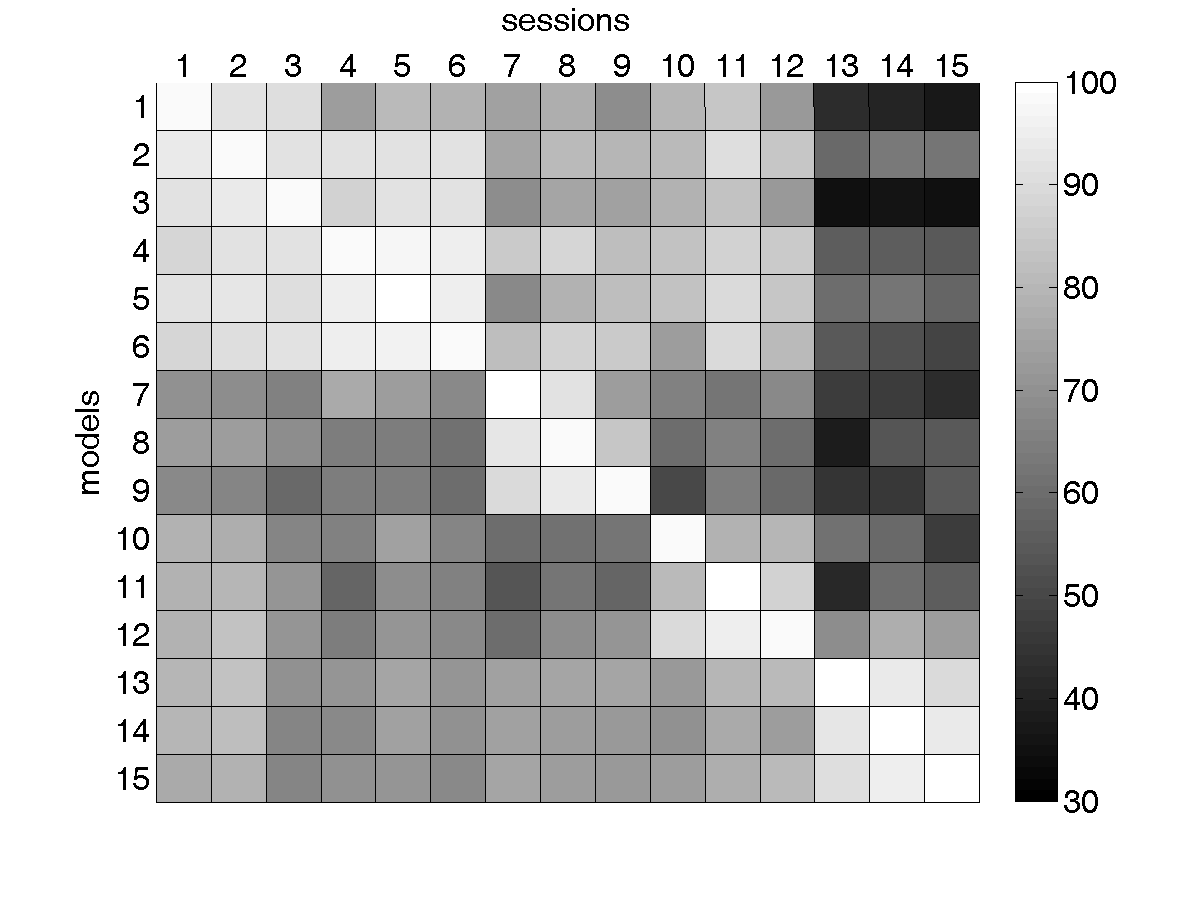
\includegraphics[width=0.45\textwidth]{figs/fig_resCross1_full} & 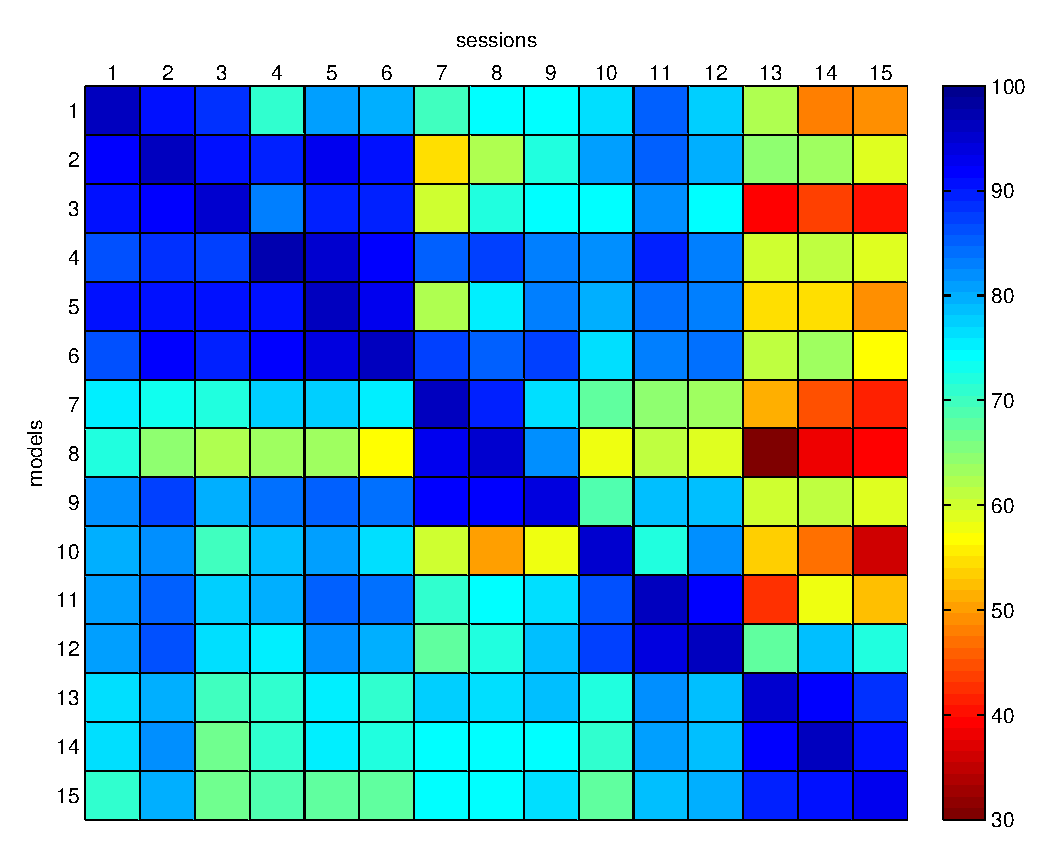
\includegraphics[width=0.45\textwidth]{figs/fig_resCross1} \\
    diagonal: $98.73\% \pm 0.39\%$  & diagonal: $95.52\% \pm 1.21\%$ \\
        rest: $73.23\% \pm 14.29\%$ & rest: $74.53\% \pm 13.70\%$ \\
    $(a)$ & $(b)$ \\
    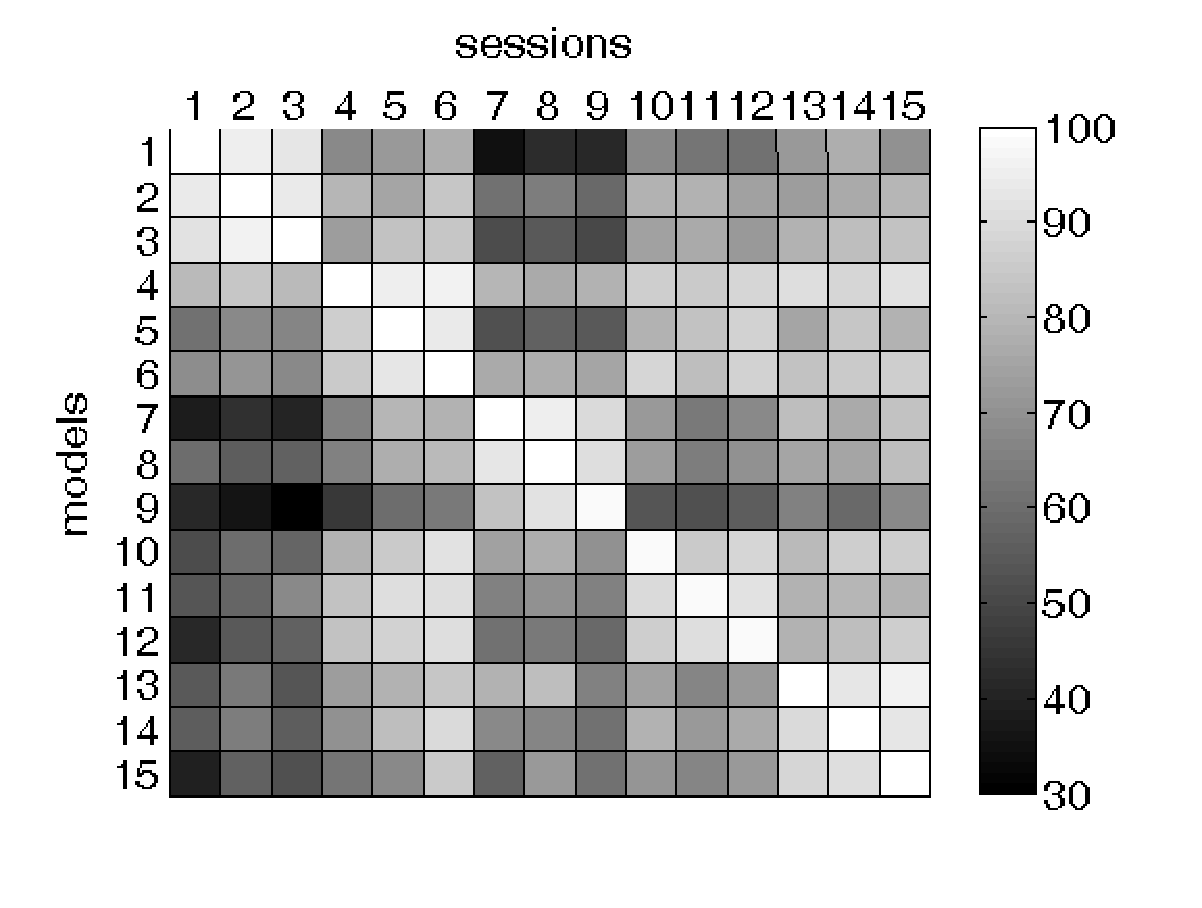
\includegraphics[width=0.45\textwidth]{figs/fig_resCross2_full} & 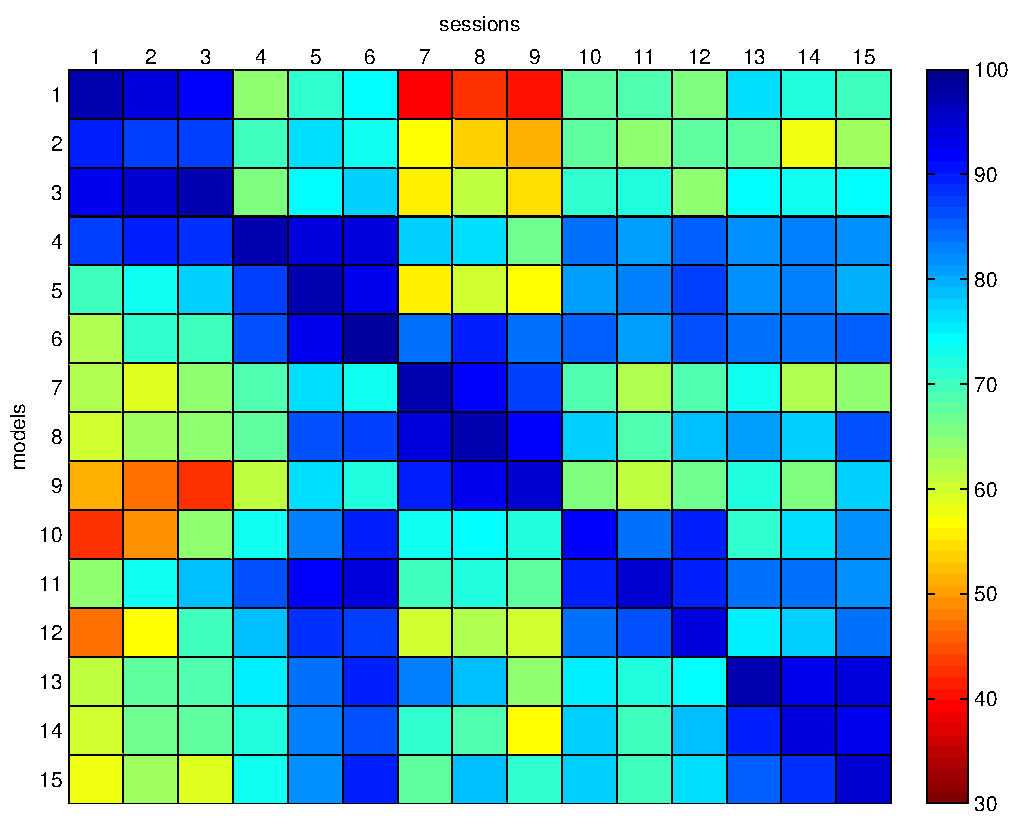
\includegraphics[width=0.45\textwidth]{figs/fig_resCross2} \\
    diagonal: $99.05\% \pm 0.37\%$ & diagonal: $95.37\% \pm 2.85\%$ \\
        rest: $73.23\% \pm 14.47\%$ & rest: $74.38\% \pm 12.27\%$ \\
    $(c)$ & $(d)$ \\
  \end{tabular}
  \caption{Cross-session analysis and evaluation of the uniformisation
    procedure. $(a)$ and $(b)$, accuracy matrices for day $1$: $(a)$
    full models, $(b)$ uniform models. $(c)$ and $(d)$, same for day $2$.}
  \label{fig:cross_initial}
\end{figure*}

Consider first panes $(a)$ and $(b)$ of the Figure, pane $(a)$ being
the accuracy matrix for full models, day $1$, and pane $(b)$ being the
accuracy matrix for the same day, but using uniform models. It is
apparent from the colours that the full models attain a better
accuracy when tested on their own training data, that is, on the
diagonal of the matrix, than the uniform models. In fact, the mean and
standard deviation of the diagonal accuracies are $98.73\% \pm 0.39\%$
for the full models and $95.52\% \pm 1.21\%$ for the uniform
models. This is intuitively sensible since, in the case of full
models, we are testing on the same data used for training, whereas in
the case of uniform models, the training data are a strict subset of
the testing data, and a quite smaller subset indeed. But as well, if
we consider the remaining elements of the matrices, it is clear that
the uniform models attain a better accuracy \emph{overall}, if
compared to the full models. In fact, the accuracies are $73.23\% \pm
14.29\%$ for the full models, and $74.53\% \pm 13.70\%$ for the
uniform ones.

The same analysis for day $2$ yields analogous results (consider the
above Figure, panes $(c)$ and $(d)$).

From this we conclude that the uniformisation procedure is effective
in reducing the training set size, without actually degrading the
performance. This is apparent from the fact that uniform models are
more accurate on testing sets which are disjoint from the training
sets. In fact, one should always ensure that this is the case, aiming
for a better generalisation error. We can say that uniform models
generalise better, at least in this case.

Therefore, from now on, all models we will be using, in the case of
SVMs and LWPR, will be the uniform ones.

\subsubsection{Classification accuracy}

Consider Figure \ref{fig:cross_initial} again, right hand side panes
($(b)$ and $(d)$) and the numbers below. The accuracy attained on
non-diagonal elements is about $74\%$, which is rather bad. One cannot
expect to correctly drive a prosthesis if one sample in four is
misclassified. At the same time, however, a strong ``good group
accuracy'' is obviously present: in each matrix, good accuracy values
are obtained on 3x3 submatrices located on the diagonals,
corresponding to cross-session accuracy for sessions \emph{belonging
to the same group}, that is, where the elastic bands were not removed
and no electrode displacement was present.

More in detail, as far as the first day is concerned (same Figure,
pane $(b)$), one can see that the first six models (trained on the
first two groups) obtain a quite good accuracy on the first six
sessions (first two groups) whereas their accuracy rapidly degrades as
more sessions are tested for. This is probably due to the first two
groups having been gathered in similar conditions, very similar
electrode positions and/or similar movements performed by the
subject. On the other hand, sessions in the last group (columns $13$,
$14$ and $15$ of the matrix) are particularly hard, except when tested
by models obtained from the last group itself --- here the effect is
probably motivated by the opposite reason: during those sessions, the
subject must have explored more relevant parts of the input
space. This is corroborated by the fact that models $13,14,15$ perform
rather well on \emph{all} sessions, if compared to other models (check
rows $13,14,15$ of the matrix). In other words, sessions $13,14,15$
contain more relevant information than the others.

Analogous considerations can be made by inspecting the accuracy matrix
of the second day, pane $(d)$ of the Figure.

From this we can confirm that \emph{electrode displacement plays a
determinant role} in the classification accuracy. Notice that muscle
fatigue seems not to enter the picture, but this is reasonable since
its effetcs are visible already within one single session (see Figure
\ref{fig:drift} again) and the machine correctly takes it into account
during the training phase. Notice once again that the uniformisation
procedure does not hinder the generalisation power of the system.

It is intuitively expected that the poor cross-session generalisation
performance is due to the problem of electrode displacement. This is
experimentally confirmed by the strong degradation in classification
accuracy among different groups. In other words, the SVM does not
generalise well when trained on a session belonging to group and
tested on a session belonging to a different group.

Poor generalisation is often due to the samples in the training and
testing sets being drawn from two different probability distributions
or from two essentially different zones of the input space. We claim
that this is the case. \textbf{[[PATRICK: I know this sounds quite
wobbly. can you say it in a more precise way, possibly with
citations?]]}

In particular, we hypothesise that the electrode displacement present
between groups (but not within a group) causes the samples in a group
to be ``shifted'' in the input space, so that testing on a different
group results in poor generalisation performance. To substantiate this
claim, we have verified that the cross-session accuracy is highly
correlated to the \emph{average minimum inter-sample distance} between
sessions. More in detail, let $S_i$ denote the training set for
session $i$; we have built a distance cross-session matrix $D$ in
which

$$ D_{ij} = \frac{1}{|S_j|} \sum_{s_j \in S_j}{\min_{s_i \in S_i}{ ||s_j-s_i||^2 } } $$

Essentially, $D_{ij}$ denotes how far away in the input space the
samples in $S_j$ are from the samples in $S_i$. Note that $D$ is in
general not symmetric, since we consider the \emph{average} of the
\emph{minimum} distance of each sample in $S_j$ from those in $S_i$.

The cross-correlation coefficient evaluated between the values of $D$
and the accuracy values of the cross-session accuracy matrix is
$-0.61$ \emph{both} for the first and the second day, indicating a
strong negative correlation. Further experiments have revealed that
this happens for Neural Networks too (cross-correlation $-0.40$ for
day $1$ and $-0.51$ for day $2$); and also, that $D$ is strongly
\emph{positively} correlated to the MSE in regression, for all the
studied approaches: $0.62/0.78$ (day $1$/day $2$) for SVMs,
$0.64/0.72$ for NNs and $0.77/0.81$ for LWPR.

In other words, the larger the distance of $S_i$ and $S_j$, the worse
the performance of model $i$ tested on session $j$, both in
classification and in regression. This tells us that $(a)$ samples of
the same group are closer to each other than sample from different
groups, therefore electrode displacement causes displacement in the
input space too; and $(b)$ that this causes bad inter-group
performance. ``Samples far away from the training set will be
predicted badly.''

In order to further sustain this claim we have checked, for each day,
that models obtained by adjoining $4$ of the $5$ groups would perform
well on the group excluded when training; this would indeed indicate
that more data is needed to train the machine, and that the required
data must somehow be found in some of (but not necessarily all) the
gathered groups. We will call these models \emph{multi-group
models}. The results are visible in Figure \ref{fig:bigmodels}.

\begin{figure*}[!ht] \centering
  \begin{tabular}{cc}
    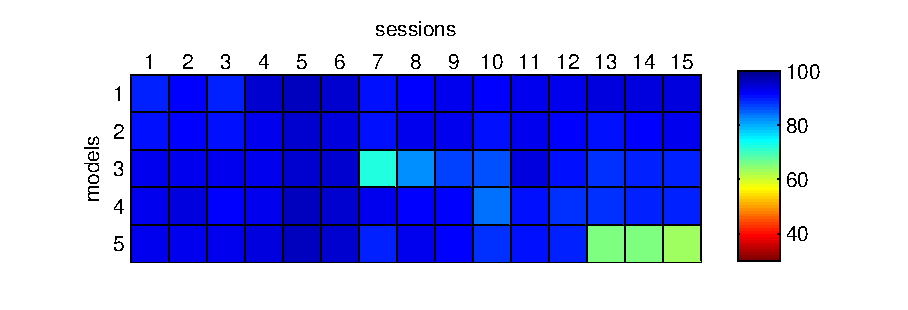
\includegraphics[width=0.45\textwidth]{figs/fig_resCross_day1_big} & 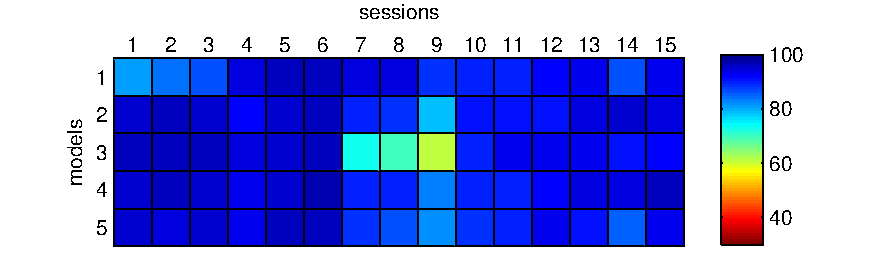
\includegraphics[width=0.45\textwidth]{figs/fig_resCross_day2_big} \\
    $(a)$ & $(b)$ \\
  \end{tabular}
  \caption{Cross-session analysis of multi-group models, obtained by adjoining $4$
    of the $5$ groups of each day. Each row denotes the model trained
    excluding group $1,\ldots,5$ from the model itself. $(a)$ day $1$, $(b)$ day $2$.}
  \label{fig:bigmodels}
\end{figure*}

Consider the rows of the matrices in the Figure: as one can see, the
accuracy is uniformly very high, even when the models are tested on
unseen testing data; for instance, model $1$ of day $1$ has an
accuracy of $92.82\% \pm 1.96\%$, and model $4$ of day $2$ has an
accuracy of $92.64\% \pm 3.73\%$. Moreover, notice that, e.g., model
$5$ of day $1$ performs badly on group $5$ of day $1$, as one can
expect, since model $5$ has not been trained on that very group, which
was already determined to be very hard (compare Figure
\ref{fig:cross_initial}, pane $(b)$, last three columns).

On the other hand, this analysis proves that if we train upon the
``right'' data, the accuracy becomes acceptable. Model $1$ of day $1$,
for instance, performs uniformly very well. From this we first
conclude that the uniformisation procedure is not eliminating any
useful information from the training sets; and, secondly, that if the
right training data can be found, there are good chances of building a
good model.

\subsubsection{Best models}

Lastly, we have considered how to collect \emph{only} relevant
information from the gathered data, that is, how to sensibly reduce
the training set. To do this, we have collected the two best models
for each day and joined them together. For instance, consider Figure
\ref{fig:cross_initial} again, pane $(b)$. It is apparent that model
$4$ performs well on sessions $1$ to $12$, whereas model $13$ does
well on sessions $13$ to $15$. We then decided to use these two models
to form a ``best'' training set which would give good results on the
whole day $1$. Analogous considerations led us to use also models $4$
and $8$ of day $2$. The obtained model will be called \emph{best}
model.

This procedure was repeated for each problem tackled (classification,
regression) and approach tested (SVM, NN and LWPR). The results are
presented below.
